\section{液体压强的公式}\label{sec:5-7}

从上节知道,液体的压强随深度而增大。但是,我们还不知道液体在任何深度的压强到底是多大。
为了解决这个问题,还需要掌握计算液体压强的公式。

\begin{wrapfigure}[12]{r}{4cm}
    \centering
    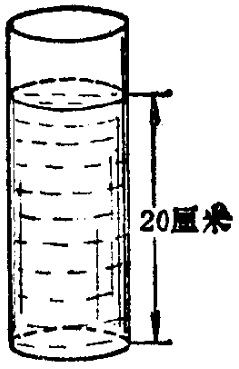
\includegraphics[width=3cm]{../pic/czwl1-ch5-23}
    \caption{}\label{fig:5-23}
\end{wrapfigure}

我们先来讨论一个具体的例子。
如图 \ref{fig:5-23} 所示,在一个底面积为 $10\pflm$ 的圆筒形容器中,盛有 20 厘米深的酒精。
我们来计算这个酒精液柱对筒底产生的压强。
酒精柱的体积是 $10\pflm \times 20\limi = 200\lflm$,酒精的密度是 $0.8\kmlflm$,
所以酒精柱的质量是 $0.8\kmlflm \times 200\lflm = 160\ke = 0.16\qianke$,
酒精柱重是 $0.16\qianke \times 9.8\ndmqk \approx 1.6\niudun$。
筒底受到的压力等于酒精柱重,筒底的面积 $10\pflm = 0.001\pfm$,因此,酒精柱对筒底的压强为
$$ \dfrac{1.6\niudun}{0.001\pfm} = 1600\pasika\;\juhao $$

上面的计算方法很容易推广到一般情况。
设想在底面积为 $S$ 的圆筒中,盛有密度为 $\rho$、深度为 $h$ 的液体,那么

液柱的体积 $V = Sh$ 。

液柱的质量 $m = \rho V = \rho Sh $。

液柱重 $G = mg = \rho gSh$。\\
这个液柱重就等于作用在底面积 $S$ 上的压力 $F$,因此深度为 $h$ 的液柱对底面的压强
$$ p = \dfrac{F}{S} = \dfrac{G}{S} = \dfrac{\rho gSh}{S} = \rho gh \,\juhao $$

上面计算的虽然只是液柱对容器的向下的压强,但是由于在同一深度处液体向各个方向的压强相等,
因此它是计算液体压强的普遍公式。


\begin{wrapfigure}[16]{r}{4cm}
    \centering
    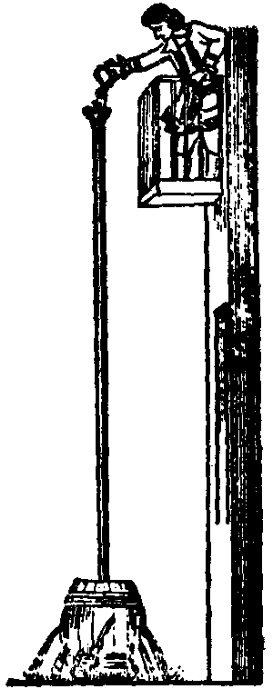
\includegraphics[width=3cm]{../pic/czwl1-ch5-24}
    \caption{}\label{fig:5-24}
\end{wrapfigure}

所以,如果用 $\rho$ 表示液体的密度,$h$ 表示液体的深度,$p$ 表示液体的压强,计算液体压强的公式就是
$$ p = \rho gh \,\juhao $$
式中的 $g$ 是一个我们用过多次的常数,等于 $9.8\ndmqk$。使用这个公式的时候,要注意只有 $h$ 用米作单位,
$\rho$ 用 $\qkmlfm$ 作单位,求出的压强单位才是帕斯卡。

值得注意的是,从液体压强的公式可以看出,液体的压强只跟深度和密度有关系,跟液体的总重和体积等都没有关系。
根据这个结论,一根细长的水柱对底面的压强,可以大大超过一大盆水对盆底的压强。这似乎是难以令人相信的。
帕斯卡为了回答当时人们的这个疑问,在 1648 年曾经表演了一个著名的实验。
他用一个密闭的装满水的木桶,在桶盖上插入一根细长的管子,从楼房的阳台上向细管子里灌水。
结果只用了几杯水,就产生了很大的压强,竟把木桶压裂了,桶里的水从裂缝中流了出来(图 \ref{fig:5-24})。
帕斯卡的实验不但生动地表明了液体压强公式的正确,而且又一次告诉人们,直觉并不一定是可靠的,
只有进行科学研究,才能够很好地认识自然规律。


\liti 油罐里装着 $4.8$ 米深的煤油,在罐壁上距罐底 $0.3$ 米处有一个小孔,用塞子塞着。
求煤油对塞子的压强。

煤油对塞子的压强就是煤油在小孔处产生的压强。

解:小孔在油面下的深度 $h = 4.8\mi - 0.3\mi = 4.5\mi$。

煤油的密度 $\rho = 0.8 \times 10^3 \qkmlfm$。利用液体压强的公式,求得煤油对塞子的压强
$$ p = \rho gh = 0.8 \times 10^3 \qkmlfm \times 9.8\ndmqk \times 4.5\mi = 3.5 \times 10^4 \ndmpfm = 3.5 \times 10^4 \pasika \,\juhao $$


\lianxi

(1) 在图 \ref{fig:5-25} 中,是 $A$ 处的压强大, 还是 $B$ 处的压强大?

\begin{figure}[htbp]
    \centering
    \begin{minipage}{5cm}
    \centering
    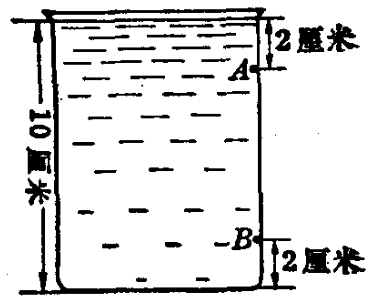
\includegraphics[width=5cm]{../pic/czwl1-ch5-25}
    \caption{}\label{fig:5-25}
    \end{minipage}
    \qquad
    \begin{minipage}{9cm}
    \centering
    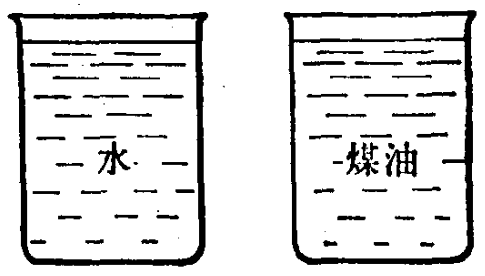
\includegraphics[width=7cm]{../pic/czwl1-ch5-26}
    \caption{}\label{fig:5-26}
    \end{minipage}
\end{figure}

(2) 在图 \ref{fig:5-26} 中,哪个容器底受到的压强较小?

(3) 在图 \ref{fig:5-24} 所示的帕斯卡实验中,如果细管的高度是 10 米,管中灌满水,水对桶上部产生的压强是多大?
管的粗细对压强有影响吗?

\begin{wrapfigure}[8]{r}{4cm}
    \centering
    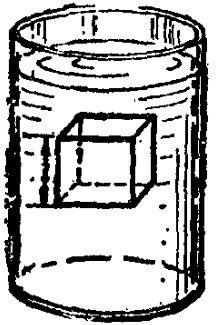
\includegraphics[width=2.5cm]{../pic/czwl1-ch5-27}
    \caption{}\label{fig:5-27}
\end{wrapfigure}

(4) 潜到海面下 50 米的潜水员,受到的海水的压强是多大?

(5) 葛洲坝水电站的拦河大坝高 70 米,当上游水位为 60 米时,坝底受到的水的压强是多大?

(6) 在竖立着的玻璃管内装着 76 厘米高的水银柱,求这段水银柱产生的压强。

(7) 一个边长为 $l$ 米的正方体,浸没在密度是 $\rho$ 的液体中,上表面在液面下 $d$ 米处(图 \ref{fig:5-27})。
正方体的上表面和下表面受到的液体的压力各是多大?方向怎样?


